\chapter{Utilisation du logiciel grâce à l'interface}\label{chap:usegraph}
  \begin{figure}[htbp]
    \centering
    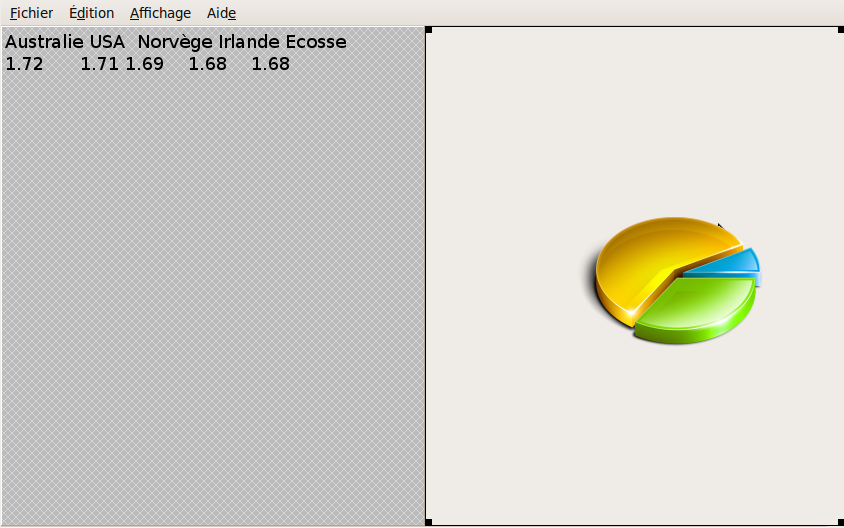
\includegraphics[scale=0.40]{img/soft}
    \caption{Apparence graphique de LoCD}
    \label{fig:apgraph}
  \end{figure}
Pour les utilisateurs peu à l'aise avec l'utilisation des commandes unix, LoCD propose un interface graphique. Bien qu'encore en developpement, cette interface permet de reprendre la plupart des fonctionalités disponibles en lignes de commandes. 
%\clearpage

%%%%%%%%%%%%%%%%%%%%%%%%%%%%%%%%%%%%%%%%%%%%%%%%%%%%%%%%%%%%%%%%%%%%%%%%%

\section{Lancement de l'application graphique}
\label{sec:lancegraph}
Si vous n'avez pas encore installé LoCD sur votre ordinateur, rendez vous à la section \ref{sec:install}. Une fois l'installion complète, il ne reste plus cliquer sur l'executable. Celui ci se trouve à l'emplacement : \verb+/.../LoCD_folder/bin/Locd+. Si un problème à lieu à ce stade, vérifiez que nous avez bien les configurations requises (\ref{sec:conf}). Pour tout autres problèmes \href{mailto:LoCD_assistance@exemple.com}{envoyez nous un mail}.

\section{Utilisation de l'interface graphique}
Voici un bref descriptif des différentes opération proposée par l'interface graphique de LoCD
\subsection{Barre des menus}
Les opérations générales sont listées dans la bare des tâches.
 \paragraph{Fichier}
 \begin{itemize}
\item
Ouvrir : Charger un ficher de données.
\item
Enregistrer : sauvegarder au format «.locd».
\item
Enregistrer sous : préciser le nom de votre sauvegarde.
\item
Exporter : Enregistrer votre diagramme au format de votre choix (pdf ou png).
\item
Quitter : Fermer l'application LoCD.
 \end{itemize} 
 
 \paragraph{Edition}
Ce menu possède le même contenu du menu contextel :
  \begin{figure}[htbp]
    \centering
    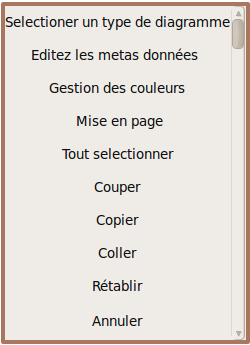
\includegraphics[scale=0.60]{img/menucont}
    \caption{Apparence du menu contextuel}
    \label{fig:menucont}
  \end{figure}

Les opérations : Selectioner un type de diagramme, Editez les metas données, Gestion des couleurs et Mise en page  effectuent les même règlages que ceus décrite dans le chapitre consacré à  l'utilisation par un terminal (\ref{chap:useterm}). Nous vous renvoyons à ce chapitre pour prendre connaissances de ces effets. La seule opération disponible exclusivement dans le menu edition est la rubrique Configuration par défault. Une nouvelle fenêtre s'ouvre et vous propose de régler des différents paramètres (couleurs, mise en page \dots) présents à la figure \ref{fig:dbatons}. 
